% Created 2015-06-13 Sat 19:37
\documentclass[11pt]{article}
\usepackage[utf8]{inputenc}
\usepackage[T1]{fontenc}
\usepackage{fixltx2e}
\usepackage{graphicx}
\usepackage{longtable}
\usepackage{float}
\usepackage{wrapfig}
\usepackage{rotating}
\usepackage[normalem]{ulem}
\usepackage{amsmath}
\usepackage{textcomp}
\usepackage{marvosym}
\usepackage{wasysym}
\usepackage{amssymb}
\usepackage{capt-of}
\usepackage{hyperref}
\tolerance=1000
\usepackage[utf8]{inputenc}
\usepackage[usenames,dvipsnames]{color}
\usepackage{commath}
\usepackage{tikz}
\usetikzlibrary{shapes,backgrounds}
\usepackage{marginnote}
\usepackage{listings}
\usepackage{color}
\usepackage{enumerate}
\hypersetup{urlcolor=blue}
\hypersetup{colorlinks,urlcolor=blue}
\setlength{\parskip}{16pt plus 2pt minus 2pt}
\renewcommand{\arraystretch}{1.6}
\author{Oleg Sivokon}
\date{\textit{<2015-06-13 Sat>}}
\title{Assignment 16, Discrete Mathematics}
\hypersetup{
 pdfauthor={Oleg Sivokon},
 pdftitle={Assignment 16, Discrete Mathematics},
 pdfkeywords={Discrete Mathematics, Assignment, Relations},
 pdfsubject={Second assignment in the course Discrete Mathematics},
 pdfcreator={Emacs 25.0.50.1 (Org mode 8.3beta)}, 
 pdflang={English}}
\begin{document}

\maketitle
\tableofcontents

\definecolor{codebg}{rgb}{0.96,0.99,0.8}
\definecolor{codestr}{rgb}{0.46,0.09,0.2}
\lstset{%
  backgroundcolor=\color{codebg},
  basicstyle=\ttfamily\scriptsize,
  breakatwhitespace=false,
  breaklines=false,
  captionpos=b,
  framexleftmargin=10pt,
  xleftmargin=10pt,
  framerule=0pt,
  frame=tb,
  keepspaces=true,
  keywordstyle=\color{blue},
  showspaces=false,
  showstringspaces=false,
  showtabs=false,
  stringstyle=\color{codestr},
  tabsize=2
}
\lstnewenvironment{maxima}{%
  \lstset{%
    backgroundcolor=\color{codebg},
    escapeinside={(*@}{@*)},
    aboveskip=20pt,
    captionpos=b,
    label=,
    caption=,
    showstringspaces=false,
    frame=single,
    framerule=0pt,
    basicstyle=\ttfamily\scriptsize,
    columns=fixed}}{}
}
\makeatletter
\newcommand{\verbatimfont}[1]{\renewcommand{\verbatim@font}{\ttfamily#1}}
\makeatother
\verbatimfont{\small}%
\clearpage

\section{Problems}
\label{sec:orgheadline20}

\subsection{Problem 1}
\label{sec:orgheadline5}
Graph \(G = (V, E)\) is defined as follows: vertex \(v \in V\) must be a subset
of cardinality exactly 3 taken from the set \(S = \{1, 2, 3, 4, 5, 6, 7\}\).
An edge \(e \in E, e = \{v_i, v_j\}\) exists only when \(\abs{v_i \cap v_j} = 1,
   v_i, v_j \in V\).
\begin{enumerate}
\item Prove that \(G\) is a connected graph.
\item Prove that \(G\) is not a bipartite graph.
\item Prove or disprove: \(G\) is an Eulerian graph.
\item Prove that \(G\) is Hamiltonian.
\end{enumerate}

\subsubsection{Answer 1}
\label{sec:orgheadline1}
Suppose, for contradiction that \(G\) is not connected, then it would have to
have two edges, call them \(v_1\) and \(v_2\) such that there isn't a path
between them.  From the definition of the graph it follows that each vertex
connects to the number of vertices that can be calculated as follows: for
each of the elements of the set assigned to the edge \(v_1\), call them \(a\),
\(b\) and \(c\), we must select such other vertices that they only contain \(a\),
but not \(b\) or \(c\).  There are clearly \(3 \cdot {7 - 2 \choose 3} = 30\) of
such edges.  Now we argue, by pigeonhole principle, that it will not be
possible to have two disconnected nodes \(v_1\) and \(v_2\) with fan-out of
30 in a graph containing all in all \({7 \choose 3} = 35\) vertices.

\subsubsection{Answer 2}
\label{sec:orgheadline2}
Recall that a bipartite graph cannot contain an odd-length cycle.  Thus,
illustrating such cycle would prove our claim.  And indeed there are such
cycles in \(G\), for instance: \((\{1, 2, 3\}, \{1, 4, 5\}, \{2, 4, 6\})\).

\subsubsection{Answer 3}
\label{sec:orgheadline3}
From definition we know that \(G\) is regular and from \ref{sec:orgheadline1} we know that
it is connected and of the degree 30.  This is sufficient to show that the
graph is Eulerian, since it is connected and every vertex has an even
degree.

\subsubsection{Answer 4}
\label{sec:orgheadline4}
Using Dirac's theorem, which states that a simple graph with \(n\) vertices
\((n \geq 3)\) is Hamiltonian if every vertex has degree \(\frac{n}{2}\) or
greater, we claim that \(G\) is Hamiltonian.  \(G\) has \(35 > 3\) vertices and
every vertex has a degree \(30 > \frac{35}{2}\).  From definition of \(G\), \(G\)
is simple since its vertices are defined to be connected if they share only
one set element, thus they can't connect to themselves (form loops), nor can
they connect to other vertices more than once.

\subsection{Problem 2}
\label{sec:orgheadline8}
\begin{enumerate}
\item Draw an Eulerian graph with even number of vertices which doesn't have a
perfect matching.
\item Prove that if \(G\) is Hamiltonian with an even number of vertices, then
it has a perfect matching.
\end{enumerate}

\subsubsection{Answer 5}
\label{sec:orgheadline6}
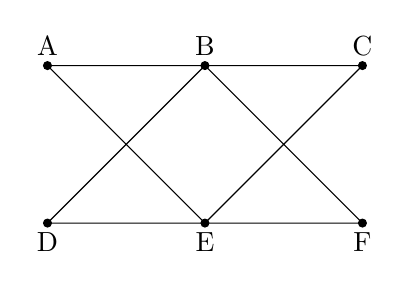
\begin{tikzpicture}
  \draw (2, 0) -- (4, 2) -- (2, 2) -- (4, 0) -- (2, 0)
  -- (0, 2) -- (2, 2) -- (0, 0) -- (2, 0);

  \draw[fill] (0, 0) circle [radius=0.05];
  \draw[fill] (2, 0) circle [radius=0.05];
  \draw[fill] (4, 0) circle [radius=0.05];
  \draw[fill] (0, 2) circle [radius=0.05];
  \draw[fill] (2, 2) circle [radius=0.05];
  \draw[fill] (4, 2) circle [radius=0.05];

  \node [below] at (0, 0) {D};
  \node [below] at (2, 0) {E};
  \node [below] at (4, 0) {F};
  \node [above] at (0, 2) {A};
  \node [above] at (2, 2) {B};
  \node [above] at (4, 2) {C};
\end{tikzpicture}

The graph is Eulerian because it has even fan-out at every vertex, it also
consists of six vertices, thus matching the requirement of having an even
number of vertices.  There is no perfect matching in this graph, which is
easy to get convinced of if you notice that it has two vertices with degree
4 viz. \(B\) and \(E\), which don't connect to each other.  In other words, both
these vertices would have to connect to every one of the remaining vertices,
thus selecting only two of the remaining four (since neithr of them can be
connected by the perfect matching to more than one vertex).  All remaining
vertices have degree 2, meaning that they don't interconnect.  Thus there is
no way to connect them pairwise without also connecting them to the vertices
with degree 4.

\subsubsection{Answer 6}
\label{sec:orgheadline7}
Having a Hamiltonian graph means having a cycle. If that cycle also happens
to have an even number of vertices, it will certainly have an odd number of
edges.  We can always order the edges in the same order they are connected
in the graph, selecting only the oddly numbered edges from this ordering will
necessarily produce a perfect matching.  It's easy to see this, because, all
vertices would be included by construction and the matching number will be
exactly half of the number of vertices, which is the definition of perfect
matching.

\subsection{Problem 3}
\label{sec:orgheadline12}
\begin{enumerate}
\item How many perfect matchings there are in \(K_5\) graph?
\item How mahy perfect matchings there are in bipartite graph \(K_{5, 5}\)?
\item Suppose we removed 4 edges from bipartite graph \(K_{5, 5}\), how many
perfect matchings there are in this graph?
\end{enumerate}

\subsubsection{Answer 7}
\label{sec:orgheadline9}
There are no perfect matchings in \(K_5\).  By definition, the number of edges
in the perfect matching must be half of the number of nodes in the graph,
but it also must be a natural number, while 5 isn't evenly divisible by 2.

\subsubsection{Answer 8}
\label{sec:orgheadline10}
Bipartite graph where each vertex in the both independent sets connects to
each vertex in the other set can be perfectly matched in the same number of
ways as many one-to-one and onto functions we can define where the cardinality
of domain and co-domain are both 5.  Or, in other words, it is the same as
the number of permutations of a sequence of length 5, viz 5!.

\subsubsection{Answer 9}
\label{sec:orgheadline11}
Similar to \ref{sec:orgheadline10}, we first count the edge between the node that has only
one edge leading to the opposite independent set, and the rest of the nodes
will only be able to choose among four remaining nodes in the opposite
independent set, thus the final answer would be \(1 + 4!\).

\subsection{Problem 4}
\label{sec:orgheadline15}
Let \(P\) be a simple path with ten nodes (i.e. a graph with two leafs and
eight nodes in between).  Graph \(G\) is defined by taking \(P\) and adding two
new nodes to it, \(v\) and \(u\), such that every node in \(P\) now connects to
both \(v\) and \(u\) and there's an edge between \(v\) and \(u\).
\begin{enumerate}
\item Show \(G\) is planar.
\item Add one more node, \(w\) and connect it to \(v\), \(u\), and to the both leafs
of \(P\).  Call this graph \(H\). Prove \(H\) isn't planar.
\end{enumerate}

\subsubsection{Answer 10}
\label{sec:orgheadline13}
In order to show that the graph isn't planar, we only need to show that it
doesn't embed neither \(K_5\) graph, nor \(K_{3, 3}\) graph.  Note that \(G\)
doesn't contain \(K_5\) because there are two nodes in it with degree 11 and
the rest are either 4 or 3, but no three nodes with degree 4 form a \(K_3\).
In other words, if we order the nodes of \(P\) starting at one leaf and adding
the node connected to the node we just counted, then no two evenly numbered
nodes are connected, neither two oddly numbered nodes are connected.  In
order to show that \(K_{3,3}\) is not a minor of \(G\), note that there are no
three vertices in \(G\) such that they would connect to three same other
vertices.  Each of the vertices in \(P\) connects to at most two of its
neighbours. As for the \(v\) and \(u\), which would be the only likely
candidates, we are one vertex short to complete to \(K_{3, 3}\).
Since neither \(K_5\) nor \(K_{3, 3}\) are \(G\)'s minors, \(G\) must be blanar.

\subsubsection{Answer 11}
\label{sec:orgheadline14}
Continuing the argument for the embedding of \(K_{5}\) as a minor of \(G\) in
\ref{sec:orgheadline13}, we see that once we add one more node and edges between the leafs
of \(P\), \(v\) and \(u\), we can now find a minor \(\{x, y, v, u, w\}\) which is a
\(K_{5}\) (\(x\) and \(y\) being the leafs of \$P\$).  The edges between \(v, u, w\)
are a given.  We are also given that \(x\) and \(y\) link to any of \(v, u, w\).
We thus only need to show that it is possible to connect \(x\) and \(y\) in a way
that doesn't involve any of \(v, u\) or \(w\).  But this is immediate from
definition of \(P\).  Hence \(H\) embeds \(K_5\) as a minor, hence it cannot be
planar.

\subsection{Problem 5}
\label{sec:orgheadline19}
\begin{enumerate}
\item What is the chromatic indes of \(P\) from \ref{sec:orgheadline15}?
\item What is the chromatic indes of \(G\) from the previous problem?
\item What is the chromatic indes of \(H\) from the previous problem?
\end{enumerate}

\subsubsection{Answer 12}
\label{sec:orgheadline16}
Since \(P\) is a path, we only need 2 colors to paint its edges.

\subsubsection{Answer 13}
\label{sec:orgheadline17}
The highest degree in \(G\) is 11, thus we would need at least so many colors
to paint it.

\subsubsection{Answer 14}
\label{sec:orgheadline18}
By similar argument, we would need at least 12 colors to paint the edges of
\(H\).
\end{document}